%% Template.tex; Solar Physics
%% 
\documentclass[namedreferences]{SolarPhysics}
%
% spr-sola-addons available options:
%  natbib        -- For citations: redefine \cite commands
%  solaenum      -- makes enumerated list with italics-roman numerals and a single right-bracket
%  linksfromyear -- loads a natbib and puts a link on a year citation (hyperref must be loaded)
%  optionalrh    -- for optional running title/author
%
\usepackage[optionalrh,solaenum]{spr-sola-addons} % For Solar Physics 
%\usepackage{epsfig}                     % For eps figures, old commands
\usepackage{graphicx}                    % For eps figures, newer & more powerfull
%\usepackage{courier}                    % Change the \texttt command to courier style
%\usepackage{amssymb}                    % useful mathematical symbols
\usepackage{color}                       % For color text: \color command
\usepackage{url}                         % For breaking URLs easily trough lines
\def\UrlFont{\sf}                        % define the fonts for the URLs


%% Local definitions
%% please place your own definitions here and don't use \def but
%% \newcommand{}{} or 
%% \renewcommand{}{} if it is already defined in LaTeX



%%%%%%%%%%%%%%%%%%%%%%%%%%%%%%%%%%%%%%%%%%%%%%%%%%%%%%%%%%%%%%%%%%
\begin{document}

\begin{article}

\begin{opening}

\title{THE HELIO 100 CME CHALLENGE}

%%%%%%%%%%%%%%%%%%%%%%%%%%%%%%%%%%%%%%%%%%%%%%%%%%%
%% Authors Names
%
\author{I.~\surname{}%$^{1}$\sep
%        I.~\surname{}$^{1}$\sep
%        I.~\surname{}$^{2}$      
       }

%%%%%%%%%%%%%%%%%%%%%%%%%%%%%%%%%%%%%%%%%%%%%%%%%%%
%% Runningheads
%
%\runningauthor{}
%\runningtitle{}


%%%%%%%%%%%%%%%%%%%%%%%%%%%%%%%%%%%%%%%%%%%%%%%%%%%
%% Affilations 
%
  \institute{$^{1}$ First affiliation
                     email: \url{e.mail-a} email: \url{e.mail-b}%\\ 
%             $^{2}$ Second affiliation
%                     email: \url{e.mail-c} \\
             }


%%%%%%%%%%%%%%%%%%%%%%%%%%%%%%%%%%%%%%%%%%%%%%%%%%%
%%% Abstract 
\begin{abstract}

Studying the propagation and impact of solar eruptive events and their various manifestations is of great importance for understanding and predicting space weather conditions in the heliosphere. The Heliophysics Integrated Observatory (HELIO) was generated out of a need to robustly link the detections of solar-driven events at different locations in space, via remote-sensing and in-situ instruments onboard various spacecrafts. Under development since 2009, HELIO is now at a stage of great scientific benefit for large-scale studies of solar and heliospheric phenomena, through the generation of workflows that use HELIO to access and cross-correlate event lists and their measured properties.

%Geomagnetic storms at Earth can cause adverse effects on global communication networks, satellite operations, and human space travel. This is of increased importance in the current era of complex global communication systems, space-based communication systems, human space travel, and especially their potentially adverse effects in the vicinity of the Earth.


The fourth HELIO coordinated data analysis workshop (HELIO CDAW-4) held in Trinity College Dublin in September 2012 outlined three challenges to be addressed by working groups comprising solar physicists and computer scientists. The challenges were titled: (1) ``Heliospheric variability over the solar cycle"; (2) ``The 100 CME challenge"; and (3) ``HELIO as a tool for space weather". In this paper we outline the success of challenge (2), that focused on using HELIO to study the origin, propagation and impacts of a large number of coronal mass ejections (CMEs) in the heliosphere. HELIO provides an interface that allows researchers to track active regions as they evolve and produce solar flares and CMEs. Once launched, CMEs can be tracked in coronagraph and heliospheric images. Their impacts throughout the heliosphere can then be measured using in-situ instruments from a number of spacecraft throughout the solar system. The aim of this challenge was to use HELIO to track a large number of CMEs that had an associated type II radio burst from their source region on the surface of the Sun, and possible flare occurrence, to their effects through interplanetary space. This was achieved through the generation of a workflow that accessed the corresponding event lists and used a ballistic CME propagation model to predict each event's arrival time at Earth and elsewhere in the solar system. This provides a timeframe for determining the in-situ parameters measured at the different spacecraft locations where a CME impact was detected, and thus allows us to combine the data across multiple spacecrafts on a per-event basis for comprehensive analysis of the physics of their propagation and evolution.


Poster:

Studying the propagation and impact of solar eruptive events and their various manifestations is of great importance for understanding and predicting space weather conditions in the heliosphere. The Heliophysics Integrated Observatory (HELIO) provides an interface that allows researchers to track coronal mass ejections (CMEs) from their source region on the Sun, to their effects in interplanetary space. The aim of this challenge was to use HELIO to track a large number of CMEs having an associated type II radio burst and possible flare site on disk, through interplanetary space via their detected impacts at various spacecrafts. This was achieved by generating a workflow that accessed the corresponding event lists and used a ballistic CME propagation model to predict each event's arrival time at the expected impact sites (e.g. L1 near Earth). This provided a timeframe for determining the in-situ parameters measured at the different spacecraft locations along the CME trajectory, and thus allowed us to combine the remote-sensing and in-situ data across multiple spacecrafts on a per-event basis for comprehensive analysis of the physics of their propagation and evolution.


\end{abstract}



%%%%%%%%%%%%%%%%%%%%%%%%%%%%%%%%%%%%%%%%%%%%%%%%%%%
%% Keywords
%
%\keywords{}


\end{opening}
%-------------------------------------------------

%%%%%%%%%%%%%%%%%%%%%%%%%%%%%%%%%%%%%%%%%%%%%%%%%%%
%% Sections
%
% \section{}%\label{s:?} 
\section{Introduction}

\begin{figure} 
\centerline{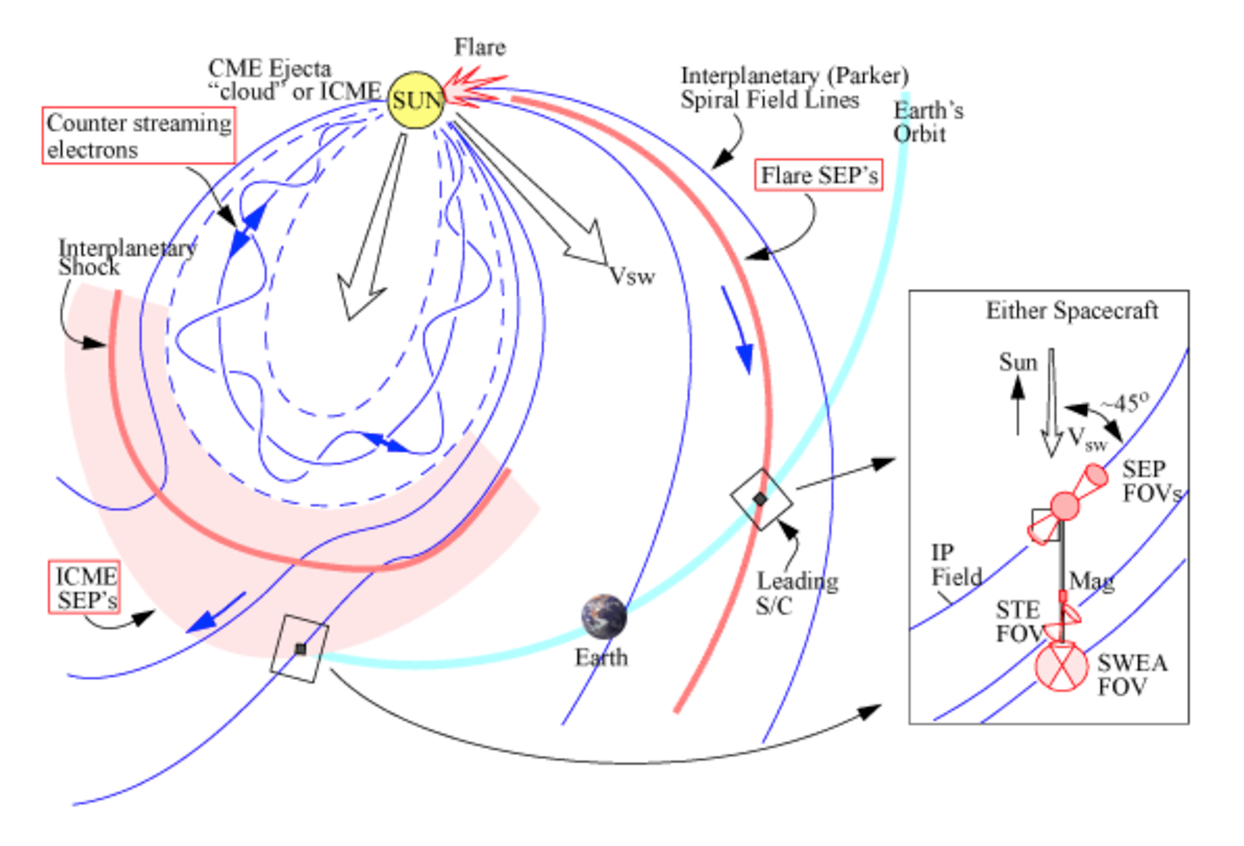
\includegraphics[width=\textwidth, clip=]{images/science_of_impact_c.pdf}}
\caption{}%\label{fig:?}
\end{figure}

\section{Building a workflow}

The challenge group began by choosing a `test case' CME for tracking through the HELIO interface, and building a model workflow to be ultimately extended for a large scale study of many events. The CME chosen was a fast event associated with a flare and type II radio burst, as listed in the ``Wind/WAVES type II bursts and CMEs" list \footnote{http://cdaw.gsfc.nasa.gov/CME\_list/radio/waves\_type2.html}. The radio burst was detected at 04:20~UT on 11~April~2004, with an associated NOAA C\,9.6 flare at disk location S\,14\,W\,47, and CME observed  in LASCO at 04:30~UT with central position angle 203$^{\circ}$, angular width 314$^{\circ}$, and speed 1645\,km\,s$^{-1}$.

The workflow was built in the following manner:

\begin{enumerate}

\item A time interval is specified and input to the ``Wind/WAVES type II bursts and CMEs" list to retrieve a list of events within the given time-range of interest.

\item From the list of candidate events, those having the fastest velocity CMEs were isolated and the top 100 chosen for the purposes of this challenge.

\item The GOES X-ray flare list was then inspected for any associated flaring activity on the disk, within a specified window of $\pm$1~hour on each event time-range.

\item Since the ``Wind/WAVES type II bursts and CMEs" list is compiled manually, the automated CACTus CME catalogue is inspected in order to associate CME parameters that carry a robust determination of their parameters. In this case the necessary parameters are the CME initial and final speeds, position angles, and angular widths. The choice of catalogue can be changed, for example to call the SEEDS catalogue instead.

\item An initial estimate of the uncertainty on the CME speed is calculated as $\sigma_v=|v_{init}-v_{final}|/2$, and a clause is put on the angular width that if it is greater than $180^{\circ}$, i.e., a halo CME, its true width is calculated as half the plane-of-sky width ($\theta^{halo}_{true}=\theta^{halo}_{pos}/2$).

\item The HELIO ballistic CME model is run with the following input parameters: start time from the peak time of the associated flare; trajectory from the associated flare longitude; speed and uncertainty estimate, and angular width (as calculated above).

\item From the ballistic CME model, an expected timeframe of arrival at the L1 point (the first Lagrangian point, near Earth) is determined. If an event is not deemed Earth-directed it is flagged as so. The in-situ data from the ACE spacecraft is queried, and an average speed of the solar wind during this timeframe is calculated. 

\item From the average solar wind speed, a new velocity of the CME is calculated to essentially account somewhat for the influence of drag. The 



\end{enumerate}





%% Figure 
%
% \begin{figure} 
% \centerline{\includegraphics[width=0.5\textwidth,clip=]{<fig.eps>}}
% \caption{}%\label{fig:?}
% \end{figure}



%% Table
%
% \begin{table}
% \caption{}%\label{tbl:?}
% \begin{tabular}{}     
% \hline
% \multicolumn{2}{c}{<>}
% <data>
% \hline
% \end{tabular}
% \end{table}
  

%%%%%%%%%%%%%%%%%%%%%%%%%%%%%%%%%%%%%%%%%%%%%%%%%%%%%%%%%%%%%%%%%%%%%%%%%%%
%% Appendix
%
% \appendix   



%%%%%%%%%%%%%%%%%%%%%%%%%%%%%%%%%%%%%%%%%%%%%%%%%%%%%%%%%%%%%%%%%%%%%%%%%%%
%% Acknowledgements
%
% \begin{acks}
%
% \end{acks}


%%% %%%%%%%%%%%%%%%%%%%%%%%%%%%%%%%%%%%%%%%%%%%%%%%%%%%%%%%%%%%
%% Bibliography
%
% Using BibTeX
%
%\bibliographystyle{spr-mp-sola}
\bibliographystyle{spr-mp-sola-cnd} %% Alternative style: no title, no concluding page
\bibliography{references.bib}  
%
% Without BibTeX 
% \begin{thebibliography}{}
% \bibitem[\protect\citeauthoryear{Author}{Year}]{key}
%   <bibliographical entry>
%
% \bibitem[\protect\citeauthoryear{}{}]{}
%   
%  
% \end{thebibliography}

\end{article} 
\end{document}
